\chapter{Discussion} \label{ch:discussion}

\section{Threshold calibration}
Different \acrshort{cam} methods exhibit different localization performance distributions, as illustrated in Fig. \ref{fig:boxacc_resnet50_imagenet}. Fixing the score map threshold at a pre-defined value, can lead to increased performance of some methods and to decreased performance for others. 

Under our threshold-independent performance measures MaxBoxAccV3, we observe that the methods have different optimal score map threshold (at maximum box accuracy) on ImageNet and the methods do not exhibit significantly different MaxBoxAccV3 performances.

\begin{figure}[ht]
    \begin{center}       
    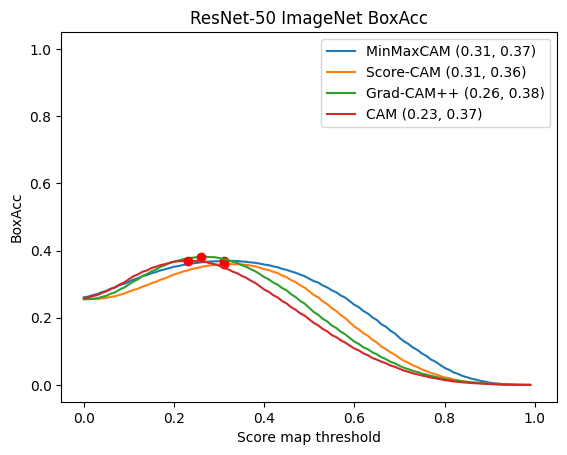
\includegraphics[width=0.7\textwidth]{fig_boxacc_resnet50_imagenet.png}
    \caption[BoxAcc for ResNet-50 on ImageNet]{Performance at varying operating thresholds. ResNet-50 on ImageNet: BoxAcc($\tau$) versus score map threshold $\tau$.}
    \caption*{Source: Author}
    \label{fig:boxacc_resnet50_imagenet}
    \end{center}
\end{figure}

\section{Classification versus localization accuracy}
In many cases, the best localization performances are achieved at early epochs, before the classifiers are sufficiently trained. We illustrate this in Fig. \ref{fig:classification_versus_localization} for the MinMaxCAM method where we show the training curves of the classification accuracy and localization accuracy on the synthetic validation dataset for the ResNet-50 network. 

\begin{figure}[ht]
    \begin{center}       
    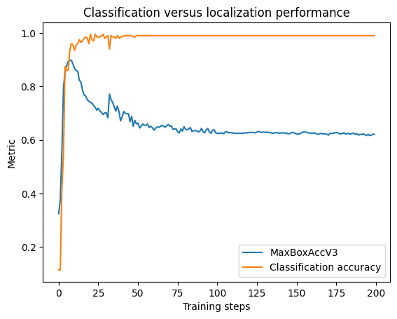
\includegraphics[width=0.7\textwidth]{fig_class_vs_localization.png}
    \caption[Classification versus localization accuracy]{Classification versus localization accuracy comparison of MinMaxCAM method for the VGG16-GAP model on the synthetic dataset.}
    \caption*{Source: Author}
    \label{fig:classification_versus_localization}
    \end{center}
\end{figure}

During the early training epochs, both classification accuracy and localization accuracy improve. But in further epochs, classification accuracy keeps improving, while localization performance drops until they both converge.

The result shows that localization and classification performance may not necessarily correlate and further classification training may hurt localization performance. As classification accuracy improves, the model focuses on learning the most discriminative parts of an object to classify the image correctly. These discriminative parts only partially cover an object. As the localization objective is to cover the full object region, improving classification performance decreases localization accuracy. 

Therefore, it's important to use localization-only metrics like MaxBoxAccV3 and PxAP for model selection and evaluation of WSOL methods. To avoid learning a model which focuses on optimizing classification performance only, we stop the learning process when the validation loss hasn't decreased for five consecutive epochs.
